\chapter{Background}

  \section{Neural Networks}
    % \begin{figure}
    %     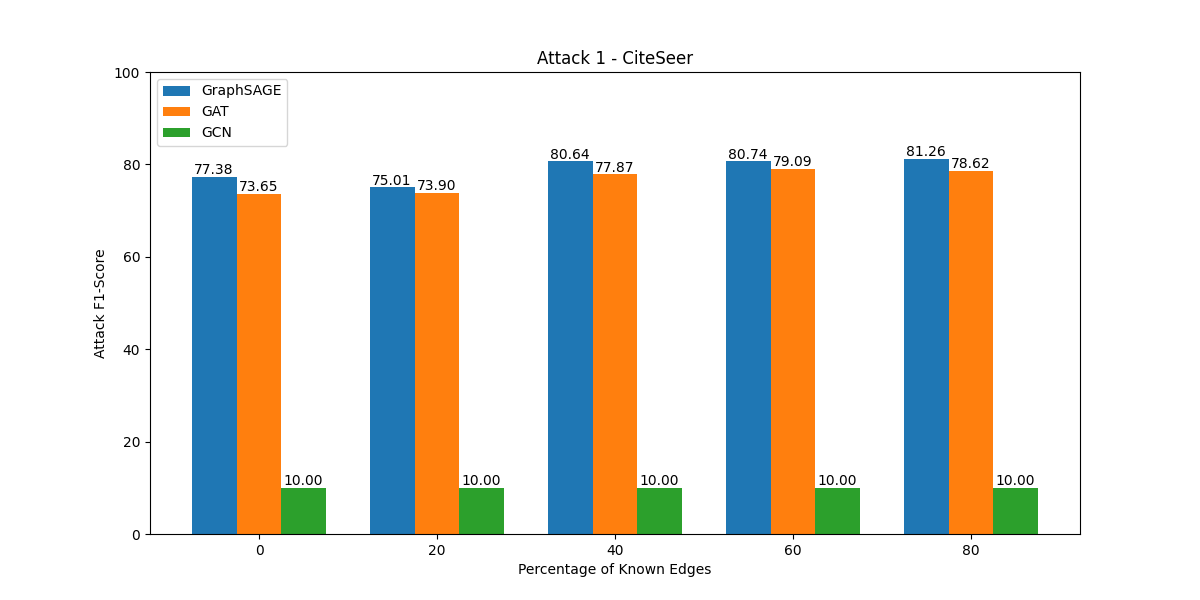
\includegraphics[scale=0.5]{res/Figures/attack-1-citeseer}
    %     \caption{This is an attacker}
    %     This is something else
    % \end{figure}

	\section{Graphs}

		As Graph we denote a data structure that contains nodes and edges. A node can have multiple attributes describing it and an edge describes the relationship between them. The most popular example where graphs are used are social networks. The nodes represent the users that have multiple attributes like location, gender, work place etc. In a directed graph user $A$ will have an outgoing edge and user $B$ an ingoing edge if $A$ follows $B$ and vice versa. In an undirected graph the edge won't have a direction. Which means that either $A$ follows $B$, $B$ follows $A$ or both will lead to the same result, namely only one edge that is drawn, describing their relationship.

	\section{Graph Neural Networks}
      
    % Describe how to query a graph neural network (f(Graph, node))

    \subsection{Transductive Learning}

    \subsection{Inductive Learning}
